\section{Background, Examples, and Goals}

A single top-level web page often incorporates multiple scripts
written by different authors.\footnote{Throughout we refer to ``web
  page'' and ``web application'' (or ``web app'') interchangeably, and
  ``JavaScript code'' and ``script'' interchangeably.} Ideally, the
browser should protect the user's sensitive data from unauthorized
disclosure, yet afford page developers the greatest possible
flexibility to construct richly featureful applications that reuse
functionality implemented in scripts provided by (potentially
distrusted) third parties. To make concrete the diversity of potential
trust relationships between scripts' authors and diverse ways page
developers may structure amalgamations of scripts, we describe several
example web applications, none of which can be implemented with strong
privacy for the user in today's web browsers. These examples
illustrate key requirements for the design of a flexible browser
confinement mechanism. Before describing these examples, however, we
offer a brief refresher on status-quo browser privacy polices.
% and a sketch of the labeling mechanism that
%forms the core of our system, \sys{}.

\subsection{Contexts and the Same-Origin Policy}
\label{sec:goals}

\paragraph{Browsing contexts}
\iffigures
\begin{figure}
\begin{center}
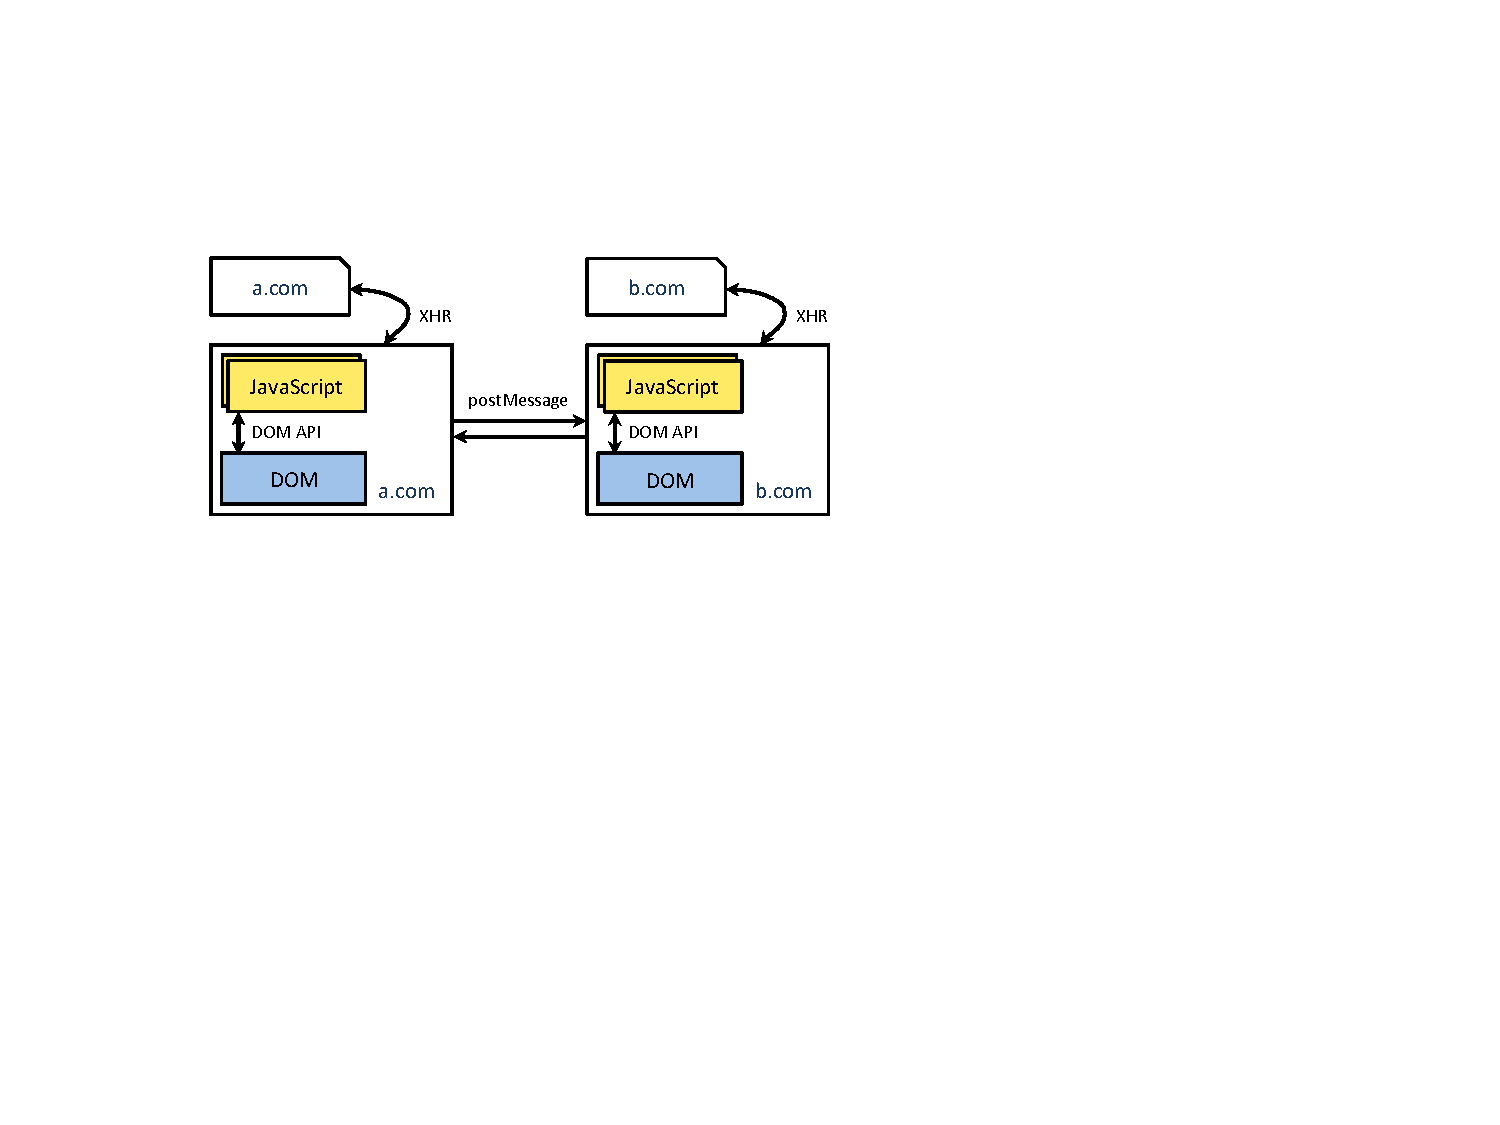
\includegraphics[width=\columnwidth]{arch.pdf}
%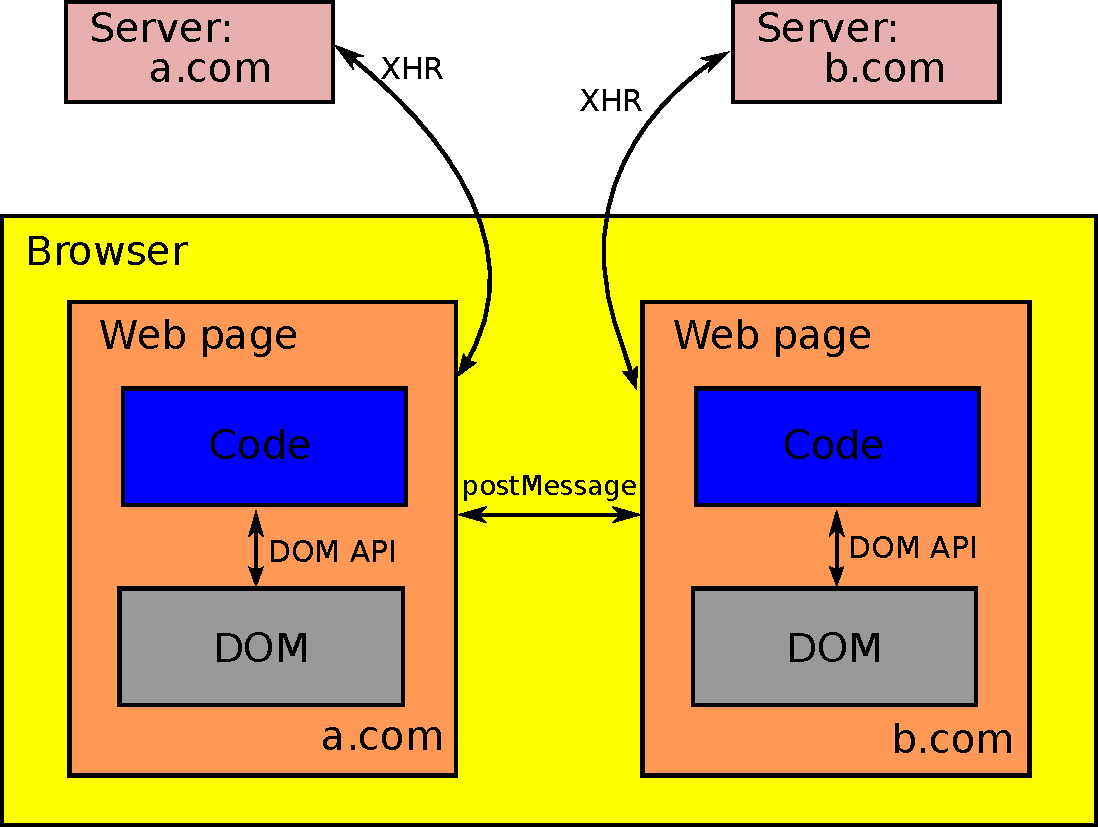
\includegraphics[scale=0.35]{setting.pdf}
\end{center}
\vspace{-10pt}
\caption{\label{fig:primer-browser-arch} Browser architecture.}
\vspace{-10pt}
\end{figure}
As shown in Figure~\ref{fig:primer-browser-arch}, a \else A \fi web page
consists of content and JavaScript code.  A \emph{browsing context}
presents a page's content to the user, and JavaScript code accesses
content within the page through the \emph{Document Object Model
  (DOM)}~\cite{html5}. Browsing contexts may be nested (e.g., by using
iframes). They also may read and write persistent storage (e.g.,
cookies) and issue network requests (either implicitly in page content
that references a URL retrieved over the network, or explicitly in
JavaScript, through invoking the \xhr{} (XHR) constructor).  Some
contexts such as Web Workers run JavaScript but do not have a DOM.

\paragraph{Origins and the Same-Origin Policy}
Since different authors may contribute components within a page,
today's status quo browsers impose a security policy on interactions
among components. Policies are expressed in terms of \emph{origins}.
An origin is a source of authority encoded by the protocol (e.g.,
\js|http|), domain name (e.g., \js|fb.com|), and port (e.g., \js|443|)
of a resource URL.\footnote{For brevity, we elide the protocol and
  port from URLs throughout, and assume that they are respectively
  \js|https| and \js|443|.}

The {\em same-origin policy} (SOP) specifies that resources of an
origin should only be readable by content from the same
origin~\cite{rfc6454, googlehandbook, VanKesteren2012}.  Browsers
ensure that code executing in an \https{a.com} context can only
inspect the DOM and cookies of another context if they share the same
(i.e., \https{a.com}) origin. Similarly, such code can only inspect
the response to a network request (performed with XHR) if the remote
host's origin is \https{a.com}.
%
%% In general, the SOP isolates code in one page from accessing client-
%% and server-side data associated with another origin.
 
The SOP does not, however, prevent code from disclosing data to
foreign origins. For example, code executing in an \https{a.com}
context can trivially disclose data to \https{b.com} by using XHR to
perform a network request; the SOP only prevents the code from
inspecting responses to such XHR requests, but does not impose any
restrictions on sending such requests.
Similarly, code can exfiltrate data by encoding it in the path of a
URL whose origin is \https{b.com}, and setting the \js|src| property
of an \js|img| element to this URL.

% More generally, the ability to embed content from an arbitrary origin
% can also be used to communicate data back into the page and ``bypass''
% the SOP's goal of disallowing cross-origin reads.
% %
% This is possible because most content is not completely opaque. 
% %
% For example, images can encode data in properties such as width and
% height (which are always readable), scripts can encode data in their
% execution sequence (as done by JSON-P~\cite{jsonp}), etc.
% %

% The popularization of JSON-P and other ad-hoc cross-origin
% communication methods, (notably, those relying on \js|window.name| and
% \js|window.location|~\cite{thidpartyjs}), has lead to the introduction
The HTML5 \js|postMessage| API~\cite{webmessaging}
allows code in different browsing contexts to exchange
messages, as shown in Figure~\ref{fig:primer-browser-arch}.
%
% Given a foreign-origin DOM window object \js|win|, the
% \js|postMessage| method can be invoked on it to send the
% foreign origin a message: \js|win.postMessage(message, destOrigin)|.
% %
% Since browsing contexts can be navigated, to prevent man-in-the-middle
% attacks~\cite{barth2009securing}, a second argument
% \js|destOrigin| is used to specify the intended origin of the message.
%
Unfortunately, a sending browsing context has no control over what a
receiving browsing context can do with the the received data. Hence in the
status quo, a developer should only send sensitive data using
\js|postMessage| if she trusts the foreign origin.
%
% in Section~\ref{sec:system:iframe}, we describe how \sys{} precisely
% allows code to impose restrictions on where the foreign-origin can
% disseminate data received via \js|postMessage|, removing this need for
% complete trust.

%\paragraph{Labels}

\subsection{Motivating Examples}
\label{sec:motivating-examples}

Having reviewed the building blocks of security policies in status-quo
web browsers, we now turn to examples of web applications for which
strong privacy is not achievable today. %the status quo. 
These examples
illuminate key design requirements for the \sys{} browser confinement
system. %, as well as the overall intuition behind its design.

\paragraph{Password Checker} Given users' propensity for choosing poor
(i.e., easily guessable) passwords, many web sites today incorporate
functionality to check the strength of a password selected by a user
and offer the user feedback (e.g., ``too weak; choose another,''
``strong,'' etc.). Suppose a developer at Facebook (at origin
\js|fb.com|) wishes to re-use password-checking functionality provided
in a JavaScript library by a third party, say, from origin
\js|sketchy.ru|. If the developer at \js|fb.com| simply includes the
third party's code in a \js|<script>| tag referencing a resource at
\js|sketchy.ru|, then the referenced script will have unfettered
access to both the user's password (provided by the Facebook page,
which the library {\em must} see to do its job) and to write to the
network via XHR. This simple state of affairs is emblematic of the
ease with which na\"{\i}ve web developers can introduce leaks of
sensitive data in applications.

A more skilled web developer could today host the checker script on
her {\em own} server and have that server specify a content security
policy (CSP)~\cite{csp} for the page that disallows scripts within the
page from initiating XHRs to any other origins. But this discretionary
access control policy is {\em too} restrictive, in that it precludes
useful operations by the checker script, e.g., retrieving an updated
set of regular expressions describing weak passwords from a remote
server (essentially, ``updating'' the checker's functionality). Doing
so requires communicating with a remote origin other than that of the
top-level page.\footnote{Unfortunately, even permitting communication
  with the top-level page's same origin is risky---a malicious script
  could then write the password to a public page at that same origin,
  in a {\em self-exfiltration attack}~\cite{selfex}.}

The key insight is that it is entirely safe and useful for an untrusted script to
communicate with remote origins {\em before} it obtains sensitive
data. We note, then, the requirement of a confinement mechanism that
allows code in a browsing context to communicate with the network {\em
  until it has been exposed to sensitive data.} MAC-based confinement
meets this requirement.

\begin{figure}
\centerline{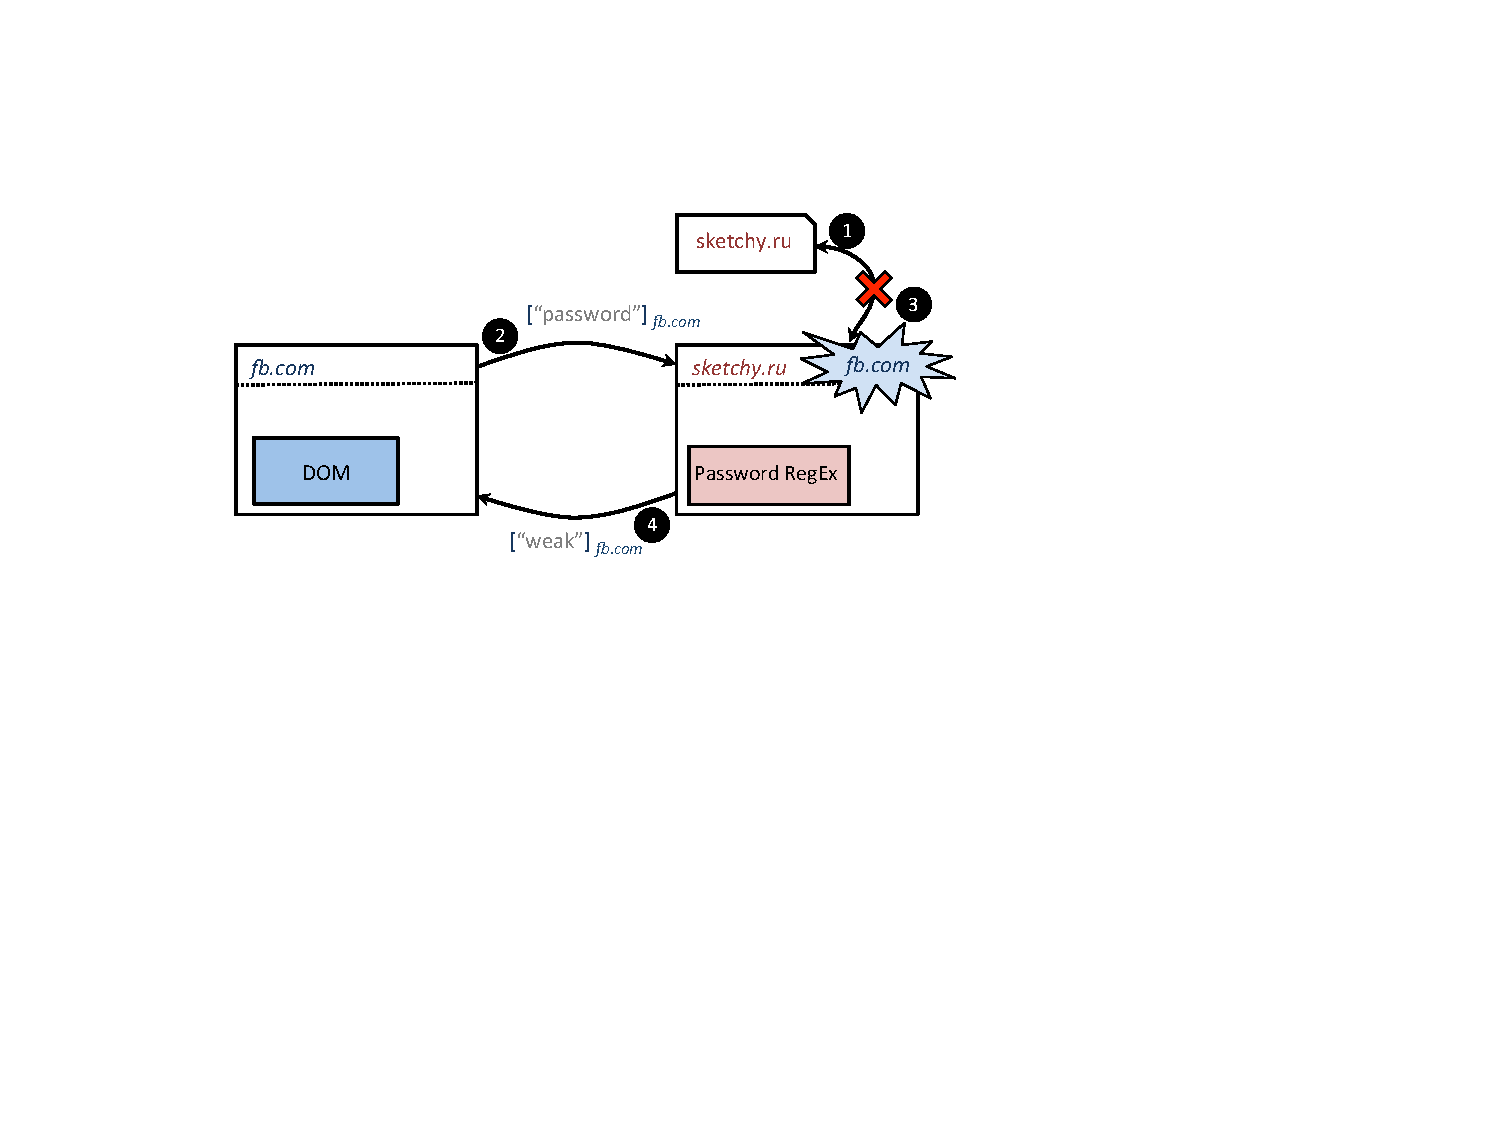
\includegraphics[width=\columnwidth]{checker}}
\caption{\label{fig:checker} Third-party password checker architecture
under \sys{}.}
\end{figure}

Figure~\ref{fig:checker} shows how such a design might look. In this
and subsequent examples, rectangular frames denote browser contexts,
arrows denote communication (either between a context and the network,
or IPC-style between contexts), and events during execution are
numbered sequentially in time. Contexts may be \emph{labeled} (Section~\ref{sec:labels}) with the
origins to whose sensitive data they have been exposed. A context that
has not yet observed sensitive data is denoted \js|public|, and a page
that contains sensitive data can \emph{raise} the label of its own
browsing context to its own origin. Here, a top-level page at
\js|fb.com| encapsulates a password-checker script from a third-party
origin within a Web Worker. Each browsing context has a
distinct current label. First, in step (1), the checker script is free
to download updated regular expressions from an arbitrary remote
origin. In step (2), the top-level page sends the user's password to
the checker script's worker using XHR\@ \todo{ar}{I thought it was via postMessage}; the browser \emph{labels} the
sent data with the origin of the page that sent it (in this case,
\js|fb.com|). When the browser delivers the password to the checker
script's context, it raises the label of the context to reflect that
the context is about to be exposed to sensitive data from \js|fb.com|. 
\Red{Consequently, and to prevent exfiltration of the sensitive data, 
\sys{} atomically denies the context further access to the network in
\Red{step (3)}.} The checker script is then
free to compute the result, which it returns via XHR to the top-level
page \Red{in step (4)}; the result carries the label \js|fb.com| to reflect that the
sender may be sending data derived from sensitive data owned by
\js|fb.com|.
% bk: unneeded to clutter this first simple example with the below, as
% other examples illustrate the need for hierarchical confinement?
%  We note further the requirement of a {\em hierarchical}
% confinement mechanism: the checker script may itself invoke untrusted
% code from still {\em other} third-party origins, and should be able to
% further confine such untrusted code.

\paragraph{Encrypted Document Editor}
%% XXX IMPORTANT bk:
%% need to articulate usage model as *company* wants to encrypt its
%% documents stored in Google Docs, and that *company* writes the
%% encryption code, which is hosted from its origin. This eliminates
%% objection, "why would the user trust the encryption library to
%% encrypt correctly, but *not* trust it not to leak the cleartext?"
Today's web applications, such as in-browser document editors backed
by cloud-based storage (e.g., Google Docs), typically require the user
to trust the app developer/cloud-based storage provider (often the
same principal under the SOP) with the data in her documents. That is,
the provider's server observes the user's data in cleartext. Suppose
an organization wished to use an in-browser document editor, but did
{\em not} want to reveal its users' document data to the editor
provider's server. How might the provider offer a privacy-preserving
editor app that would satisfy the needs of such a privacy-conscious
organization?  One promising approach might be for the ``customer''
privacy-sensitive organization to implement a trusted document encryption
service hosted at its own origin, distinct from that which hosts the
editor app. The editor app could allow the user to specify a JavaScript
``plugin'' library she trusts to perform cryptography correctly. In this design,
one origin serves the JavaScript code for the editor app (say,
\js|google.com|) and a different origin serves the JavaScript code for
the cryptography library (say, \js|nsa.gov|). Note that these two
origins may be {\em mutually distrusting.}  \js|google.com|'s script
must pass the document's cleartext to a script from \js|nsa.gov| for
encryption, and would like to confine the execution of the encryption
script so that it cannot exfiltrate the document to any origin {\em
other} than \js|google.com|. And \js|nsa.gov|'s cryptography library
does not trust \js|google.com| with the cleartext document---it would
like to confine \js|google.com|'s editor script to prevent
exfiltration of the cleartext document to \js|google.com| (or to any
other origin). This simple use case highlights the need for {\em
  symmetric confinement:} when two mutually distrusting scripts from
different origins communicate, {\em each must be able to confine the
  other's further use of data it provides the other.}

%% brings up the requirement of *symmetric* confinement: two mutually
%% distrusting origins each confine the other.

\paragraph{Third-Party Mashup}
Some of the most useful web applications are {\em mashups,} which
integrate and compute over data hosted by multiple origins. For
example, consider an application that reconciles a user's Amazon
purchases (the data for which are hosted by \js|amazon.com|) against a
user's bank statement (the data for which are hosted by
\js|chase.com|). The user may well deem both these categories of data
sensitive, and furthermore, will not want data from Amazon to be
exposed to her bank or vice-versa, nor to any other remote
party. Today, if one of the two providers implements the mashup, its
application code must bypass the SOP to allow sharing of data across
origin boundaries, e.g., by communicating between iframes with
\js|postMessage|. This approach forfeits robust confinement: one
origin sends sensitive data to the other, after which the receiving
origin may exfiltrate that sensitive data at will. Alternatively, a
third-party developer may wish to implement and offer this mashup
application. But users of such a {\em third-party mashup} give up
their privacy, as again today's browser enforces no policy that
confines the sensitive data the mashup's code observes within the
browser. To enable third-party mashups that do not sacrifice the
user's privacy, we note again the need for an untrusted script to be
able to issue requests to multiple remote origins (e.g., Amazon and
the bank), but to lose the privilege to communicate over the network
once it has read the responses from those origins.\footnote{The
  desired semantics here can be subtle. Once a third-party script
  communicates with a \emph{second} origin, should it retain the
  ability to communicate with the origin from which it \emph{first}
  read sensitive data? In some cases, allowing such communication
  would create the risk of cross-site request
  forgery~\tocite{CSRF}. We explain the correct semantics in detail in
  Section~\ref{sec:labeled-xhr}.} \Red{Deian, please check footnote; I
  have edited it for clarity, but want to make sure I've not damaged
  correctness. -BK} Here, too, MAC-based confinement meets this need.

\paragraph{Untrusted Third-Party Library}
Web application developers today make extensive use of third-party
libraries like jQuery (whose prevalence we cite in the
introduction). Simply importing a library into a page provides no
isolation whatsoever between the untrusted third-party code and any
sensitive data within the page. Developers of applications that
process sensitive data want the convenience of reusing popular
libraries. But such reuse risks exfiltration of sensitive data by
these untrusted libraries. Note that because jQuery requires access to
the content of the entire page that uses it, we cannot isolate jQuery
in a separate context from the page's context, as we did for the
password-checker example. Instead, we observe that jQuery demands a
design that is a mirror image of that for confining the password
checker: we place the {\em trusted} code for a page in a separate
context and deem the rest of the page (including the untrusted jQuery
code) as untrusted. The trusted code can then communicate with remote
origins and inject sensitive data into the untrusted page, but the
untrusted page (including jQuery) cannot communicate with remote
origins (and thus cannot exfiltrate sensitive data within the
untrusted page). Once more, MAC-based confinement intuitively seems to
fit this scenario well. We note further that any {\em library} author
may wish to reuse functionality from another untrusted
library. Accordingly, to allow the broadest reuse of code, the browser
should support {\em hierarchical confinement}---the primitives for
confining untrusted code should allow not only a single level of
confinement (one trusted context confining one untrusted context), but
arbitrarily many levels of confinement (one trusted context confining
an untrusted one, that in turn confines a further untrusted one,
etc.).

%% describe trusted compartment between page w/JQuery and network as
%% firewall---its job is to deny network requests to origins other
%% than those that are trusted.

%% after discussion with Deian:
%% there are two versions of this scenario.
%%
%% (1) page initially includes sensitive data. so steps are:
%%      (a) page creates worker with DOM access and privilege
%%      (b) page raises label to a.com; hereafter page cannot talk to
%%      any origin but a.com (so cannot leak elsewhere).
%%      (c) tcb code (in worker) loads jquery and injects it into page
%%      (d) jquery is now in page, and cannot leak
%%
%% (2) page initially includes no sensitive data, so steps are:
%%      (a) page has public label
%%      (b) page creates worker with DOM access and privilege
%%      (c) page drops privilege
%%      (d) page loads jquery (note label not raised yet!)
%%      (e) hereafter, page can only send to a.com and worker
%%      (f) worker only allows flows to allowed origins
%%      (g) tcb code transfers sensitive data from a.com, proxies into
%%      page
%%
%%  in both cases, untrusted jquery runs in page, but cannot leak to
%%  non-a.com origins.

\subsection{Design Goals}

We have briefly introduced four motivating web applications that
achieve rich functionality by combining code from one or more
untrusted parties. The privacy challenges that arise in such
applications are unfortunately unaddressed by status-quo browser
security policies, such as the SOP. These applications clearly
illustrate the need for robust yet flexible confinement for untrusted
code in browsers. To summarize, these applications would appear to be
well served by a confinement system that:

\begin{itemize}
\item applies mandatory access control (MAC);
\item supports {\em symmetric confinement,} i.e., permits two principals to {\em
    mutually} distrust one another, and each prevent the other from
  exfiltrating its data;
\item allows {\em hierarchical confinement,} i.e., permits principal
  $A$ to confine code from principal $B$ that processes $A$'s data,
  while principal $B$ can independently confine code from principal
  $C$ that processes $B$'s data, and so on.
\end{itemize}
